\title{Test Case 3 - Fluids Labs}
\author{
        Sergio M. Vanegas A.\\
        Francesco de Pas\\
                Department of Mathematics\\
        Polimi---Politecnico di Milano\\
        Milano, Italia
}
\date{\today}

\documentclass[12pt]{article}

\usepackage{amsmath}
\usepackage{graphicx}
\usepackage{siunitx}

\begin{document}
\maketitle

\begin{abstract}

        The present case concerns the development of the boundary layer produced by a uniform flow over a flat plate. The flow develops from a condition of uniform velocity \( U_\infty \) imposed at the inlet boundary, growing indefinitely without reaching a fully-developed state. Up to a distance \(x_{\text{lam}}\) from the leading edge such that \( \text{Re}_x = U_\infty x_{\text{lam}} / \nu \approx \num{1E5} \) , the boundary layer remains laminar; beyond a distance \( x_{\text{turb}} \) from the leading edge such that \( \text{Re}_x = U_\infty x_{\text{turb}} / \nu \approx \num{3E6} \) , the boundary layer is fully turbulent; in-between \( x_{\text{lam}} \) and \( x_{\text{turb}} \), transitional boundary layer will occur. In this Laboratory, PHOENICS is used to simulate the development of the laminar boundary layer, whereas the analysis of the turbulent part will be shelved for further individual study. \cite{FL:04}

        \begin{figure}[ht!]
                \centering
                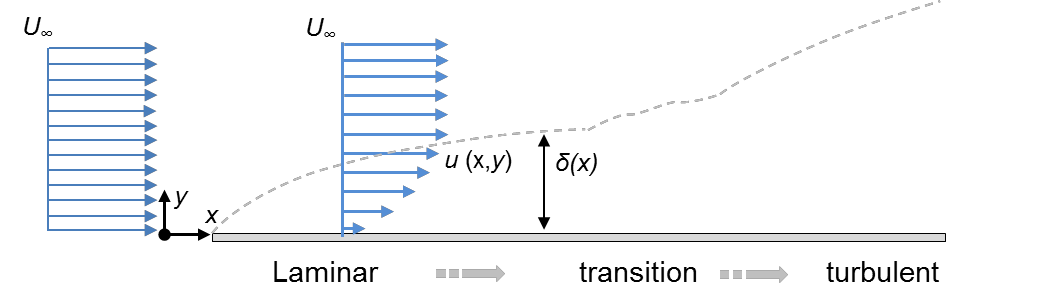
\includegraphics[width=\textwidth]{Sketch.png}
                \caption{Sketch of the test case}
                \label{fig:sketch}
        \end{figure}

\end{abstract}

\section{Introduction}

        \subsection{Reference Solution: Laminar Boundary Layer}

                Up to a distance from the leading edge \( x_\text{lam} \), corresponding to \( U_\infty x_\text{lam} / \nu \approx 1E5 \), a reference semi-analytical solution was obtained by Blasius. This solution expresses the fluid dynamic characteristics of the boundary layer as a function of the dimensionless parameter $ \eta = y \sqrt{\frac{U_\infty}{\nu x}}$, as follows:

                \begin{itemize}
                        \item U-velocity
                                \begin{equation*}
                                        \frac{u}{U_\infty} = f'(\eta)
                                \end{equation*}
                        \item V-velocity
                                \begin{equation*}
                                        \frac{nu}{U_\infty} \sqrt{\frac{U_\infty x}{\eta}} = \frac{1}{2} \left[ \eta f'(\eta) - f(\eta) \right]
                                \end{equation*}
                \end{itemize}

                From Blasius’ solution, it is also possible to obtain the following other parameters:

                \begin{itemize}
                        \item Wall shear-stress
                                \begin{equation*}
                                        \tau_w(x) = 0.332 \rho U_\infty^2 \text{Re}_x^{-\frac{1}{2}}
                                \end{equation*}
                        \item Skin-friction coefficient
                                \begin{equation*}
                                        C_f(x) = \frac{\tau_w(x)}{\frac{1}{2} \rho U_\infty^2} = 0.664 \text{Re}_x^{-\frac{1}{2}}
                                \end{equation*}
                        \item Boundary layer thickness based on the condition $ 0.99 U_\infty $
                                \begin{equation*}
                                        \frac{\delta(x)}{x} = 5 \text{Re}_x^{-\frac{1}{2}}
                                \end{equation*}
                        \item Displacement thickness
                                \begin{equation*}
                                        \frac{\delta^*(x)}{x} = \frac{\int_0^\infty \left( 1 - \frac{u}{U_\infty} \right) dy}{x} = 1.7208 \text{Re}_x^{-\frac{1}{2}}
                                \end{equation*}
                        \item Momentum thickness
                                \begin{equation*}
                                        \frac{\Theta^*(x)}{x} = \frac{\int_0^\infty \frac{u}{U_\infty} \left( 1 - \frac{u}{U_\infty} \right) dy}{x} = 0.664 \text{Re}_x^{-\frac{1}{2}}
                                \end{equation*}
                \end{itemize}

        \subsection{Flow Domain}

                A possible sketch of the computational domain is shown in Figure~\ref{fig:domain}. As for the earlier test cases, the inlet should not be placed in direct contact with the plate to avoid numerical issues at the bottom-left corner.

                \begin{figure}[ht!]
                        \centering
                        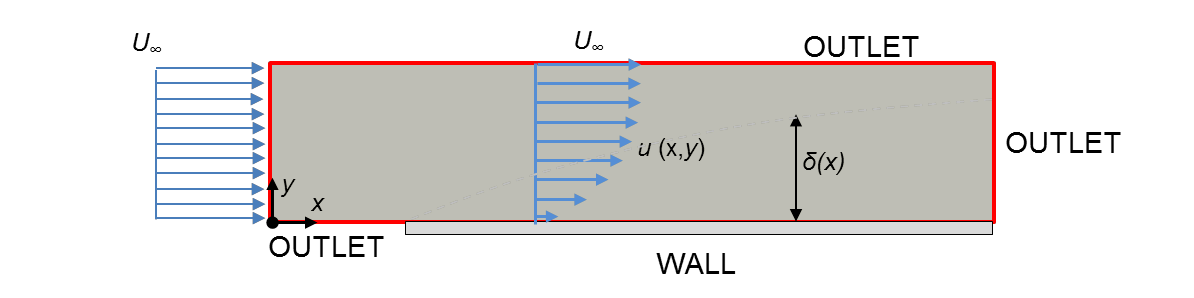
\includegraphics[width=\textwidth]{Domain.png}
                        \caption{Computational domain and Boundary Conditions}
                        \label{fig:domain}
                \end{figure}

                Since the attention is restricted to the laminar boundary layer, the steady-state formulation of the Navier-Stokes equations can be solved. When defining the CFD model particular attention must be paid in choosing the proper boundary conditions, which are, in this case, inlet, outlet, solid walls and symmetry. Let us assume no gravity. Since the flow is incompressible, gravity does not have a direct effect on the velocity field, but it just brings about a hydrostatic contribution to the pressure field.

                \begin{itemize}
                        \item At the inlet, a uniform x-velocity profile equal to \( U_\infty \) is imposed, whereas the y and z velocity components are specified as zero.
                        \item At the outlet boundaries, a zero external \( p \) is imposed. Note that the value of \( p \) at the outlet will not be zero owing to the presence of a finite outlet coefficient. In order to have $ p_\text{outlet} = p_\text{ext} = 0 $, set the outlet coefficient to a very large value (e.g. $ \num{1E10} $). This is not really necessary though.
                        \item At the solid wall, owing to the no-slip condition, the fluid velocity is zero. In the Finite Volume Framework with staggered-grid arrangement, only the y-velocity at the wall is imposed. The no-slip condition is imposed for the x-velocity indirectly. On the one hand, the advection flux of variable \( u \) through the near-wall cell faces is set to zero. On the other hand, the diffusion flux of variable \( u \) through the near-wall cell faces (that is, the wall shear-force) is specified by obtaining the wall shear-stress from the laminar friction coefficient.
                \end{itemize}

        \subsection{configuration of the problem}

                \begin{itemize}
                        \item Free-stream velocity is \( U_\infty = \SI{1E0}{\metre \per \second} \)
                        \item Workinf fluid is air at \( \SI{2E1}{\celsius} \), treated as incompressible\\(\( \rho = \SI{1.189}{\kilogram \per \metre \cubed} , \nu = \SI{1.5445E-5}{\metre \squared \per \second} \))
                \end{itemize}

        \subsection{Document Structure}

                The remainder of the report is organized as follows: Section~\ref{sec:suitability} addreses the general procedure of simulation convergence verification and mesh suitability, whereas Section~\ref{sec:comparison} compares the simulation results against the reference model.

\section{Suitability of the CFD model} \label{sec:suitability}

        In order to keep the flow within the Laminar BL, we set a domain length of \( L = \frac{\num{1E5} \nu}{U_\infty} = \SI{1.5445}{\metre} \) (with an additional \( \SI{1E-1}{\metre} \) at the beginning for computational padding). The channel height was instead qualitatively reduced until just a relatively small padding remained between the observable limit of the boundary layer and the top of the domain; the resulting height was of \( \SI{5E-2}{\metre} \).

        Since pressure was not a variable of interest for this test case, its grid independence was not studied; in its stead, both the x and y-velocity profiles at the penultimate cell were analyzed for different cell configurations, resulting in the curves observed in Figure~\ref{fig:u_ind} and Figure~\ref{fig:v_ind}.

        \begin{figure}[ht!]
                \centering
                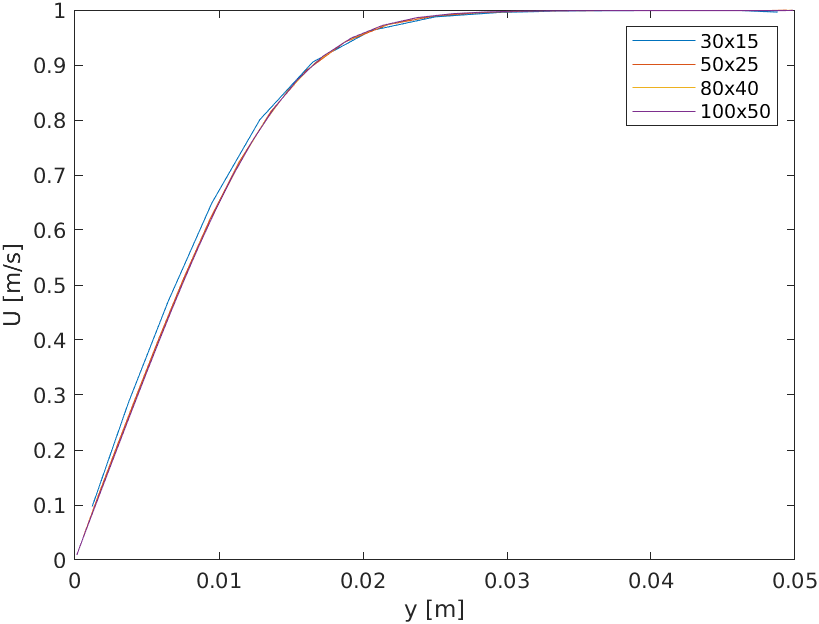
\includegraphics[width=\textwidth]{u_independence.png}
                \caption{X-velocity grid-independence study}
                \label{fig:u_ind}
        \end{figure}

        \begin{figure}[ht!]
                \centering
                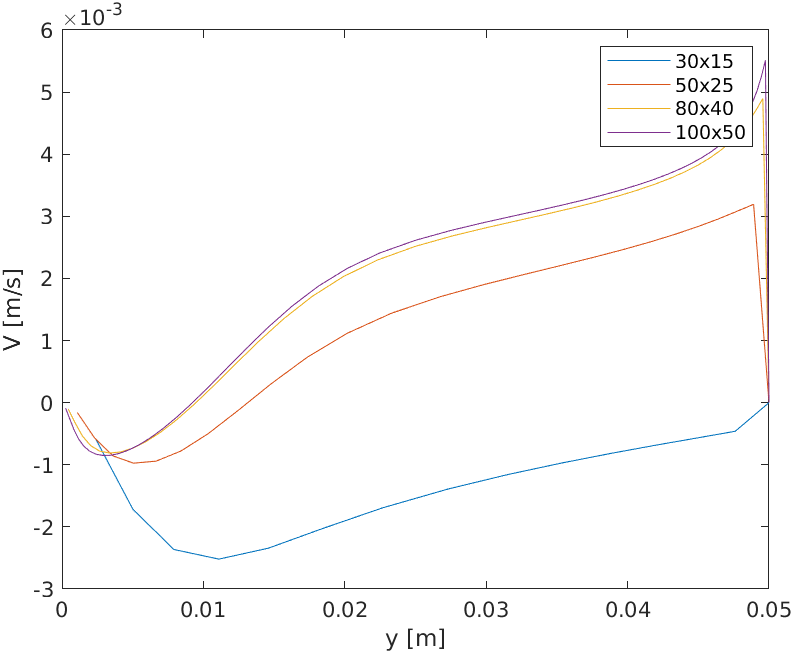
\includegraphics[width=\textwidth]{v_independence.png}
                \caption{Y-velocity grid-independence study}
                \label{fig:v_ind}
        \end{figure}

        Once grid-independence was confirmed, we decided to use the most refined configuration (100x40 cells in region of study).

\section{Comparison against the Blasius solution} \label{sec:comparison}

        

\bibliographystyle{abbrv}
\bibliography{main}

\end{document}
